\documentclass[12pt,a4paper,oneside]{article}
\usepackage[colorlinks=true]{hyperref}
\usepackage[utf8]{inputenc}
\usepackage[czech]{babel}
\usepackage{graphicx}
\usepackage{pdfpages}
\textwidth 16cm \textheight 25cm
\topmargin -1.3cm 
\oddsidemargin 0cm
\pagestyle{empty}
\begin{document}
\title{Distributor hodin CLKHUB02A}
\author{Jakub Kákona, kaklik@mlab.cz}
\maketitle

\thispagestyle{empty}
\begin{abstract}
Budič přesných digitálních hodin. Výstupy jsou v logice LVPECL vyvedené na deset SATA konektorů. Vstup signálu může být LVPECL nebo LVDS, případně pro nízké frekvence i CMOS. Budič je použitelný do frekvence 3,5GHz. 
\end{abstract}

\begin{figure} [htbp]
\begin{center}
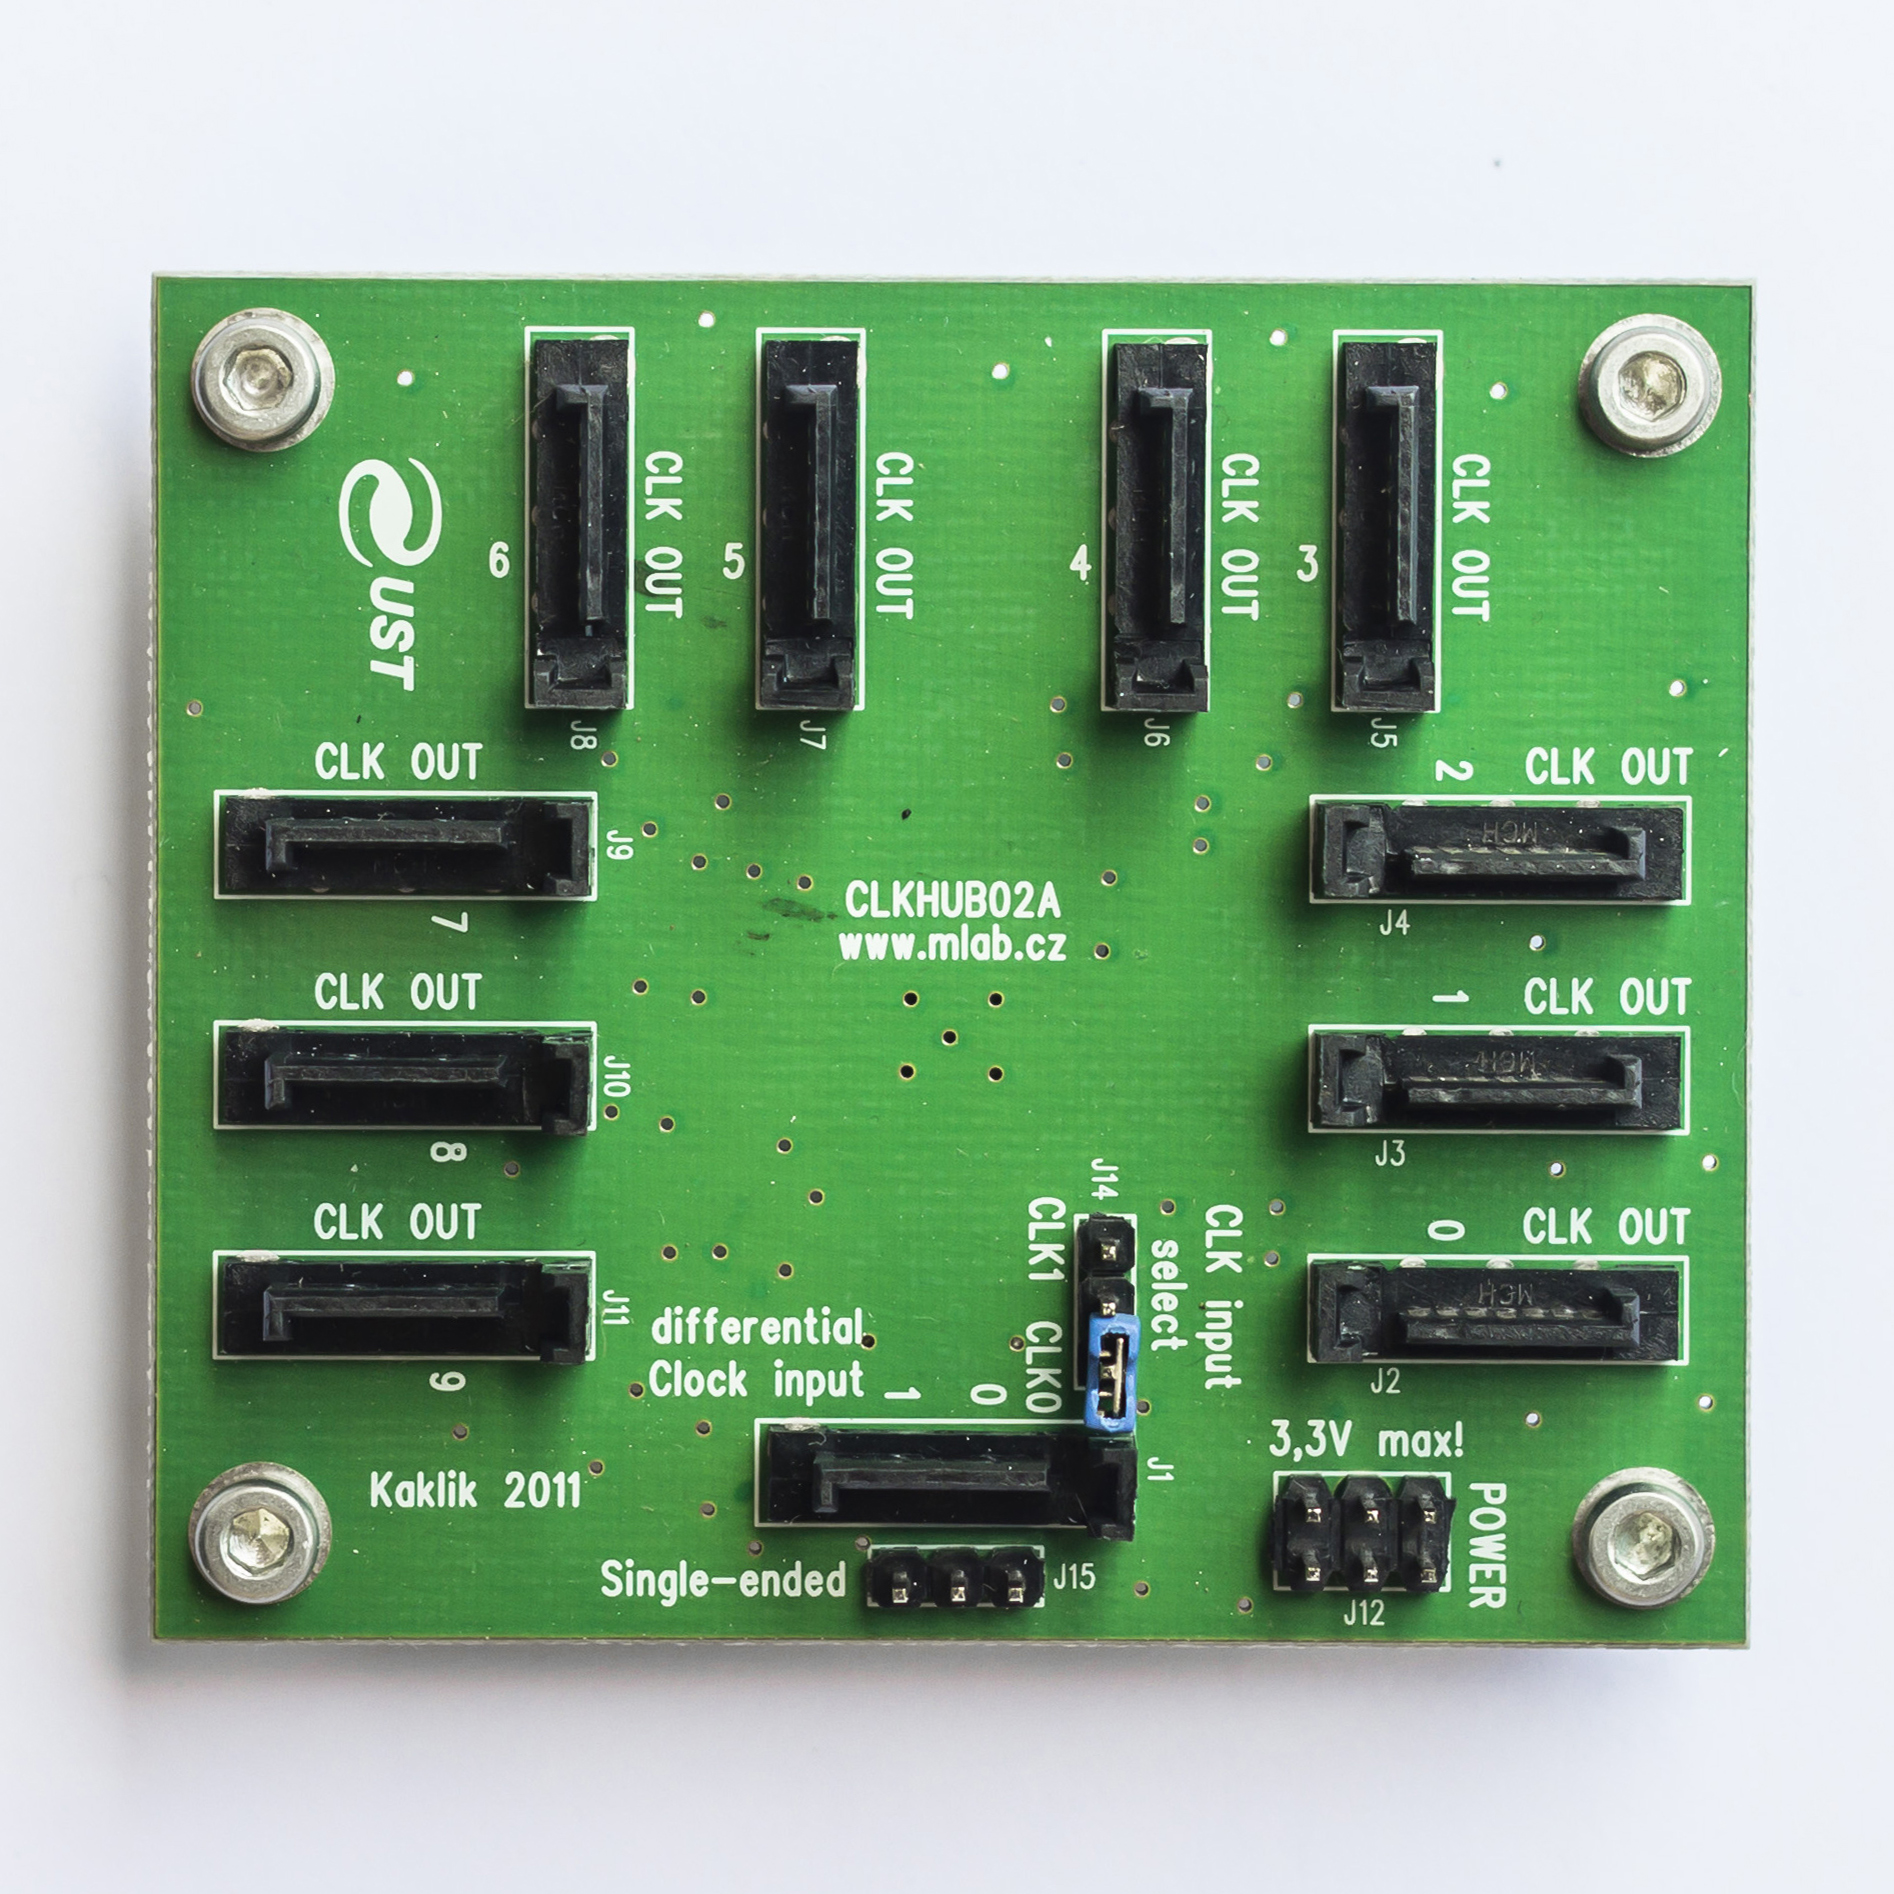
\includegraphics [width=80mm] {CLKHUB02A_Top_Big.JPG} 
\end{center}
\end{figure}

\tableofcontents

\section{Technické parametry}
\begin{table}[htbp]
\begin{center}
\begin{tabular}{|c|c|p{4.7cm}|}
\hline
Parametr & Hodnota & Poznámka \\
\hline
Napájecí napětí & max 3,3V &  Záleží na konkrétním typu logiky \\ 
\hline
Frekvenční rozsah  & 0 - 3500 MHz &  \\ 
\hline
Jitter výstupní hrany jednoho budiče & $<$ 0,3ps &  \\ 
\hline
\end{tabular}
\end{center}
\end{table}

\section{Popis konstrukce}
\subsection{Zapojení}

Modul předpokládá stabilizované napájení 3,3 V přivedené na standardní napájecí konektor.

\begin{figure} [h!tbp]
  \centering
  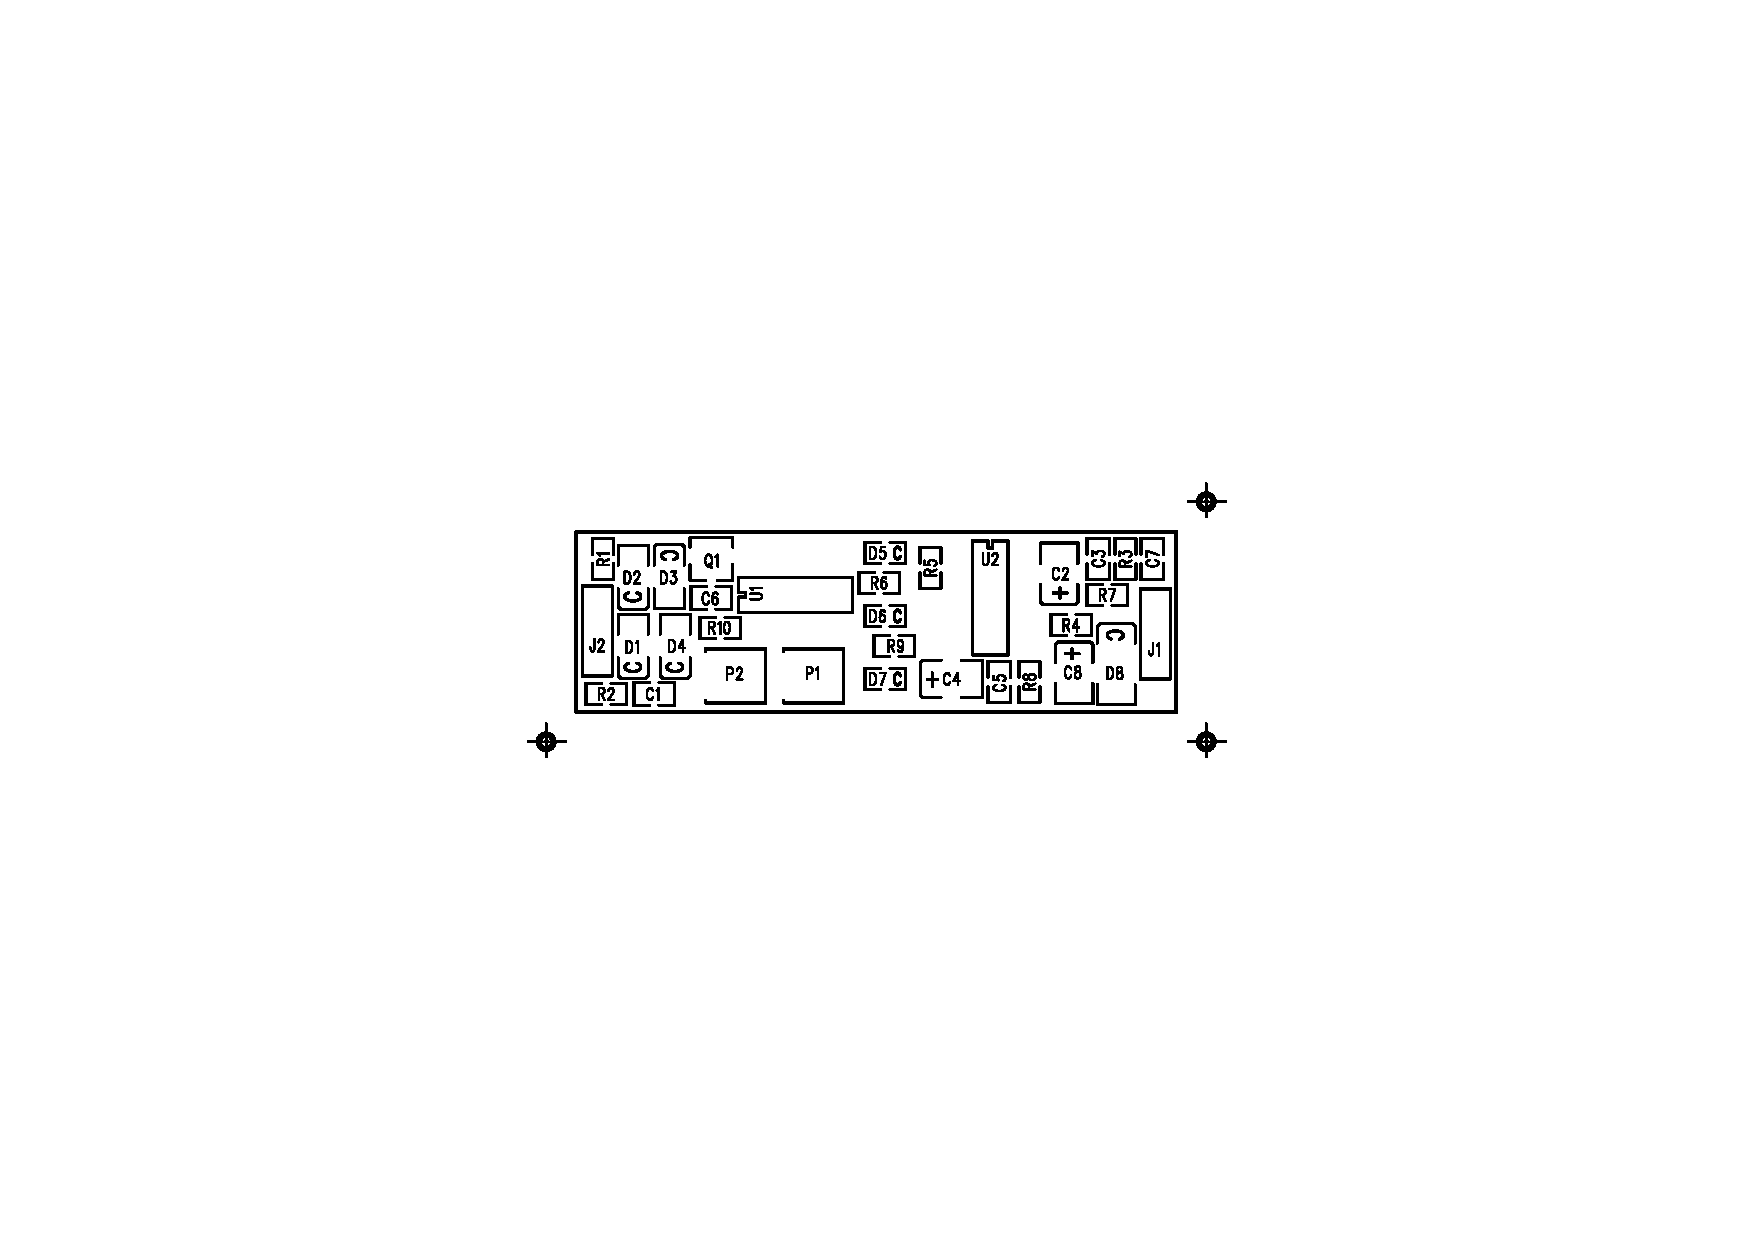
\includegraphics[trim = 6.5cm 11.5cm 6.5cm 11.5cm, clip, width=10cm]{../../CAM_DOC/O1.pdf}
  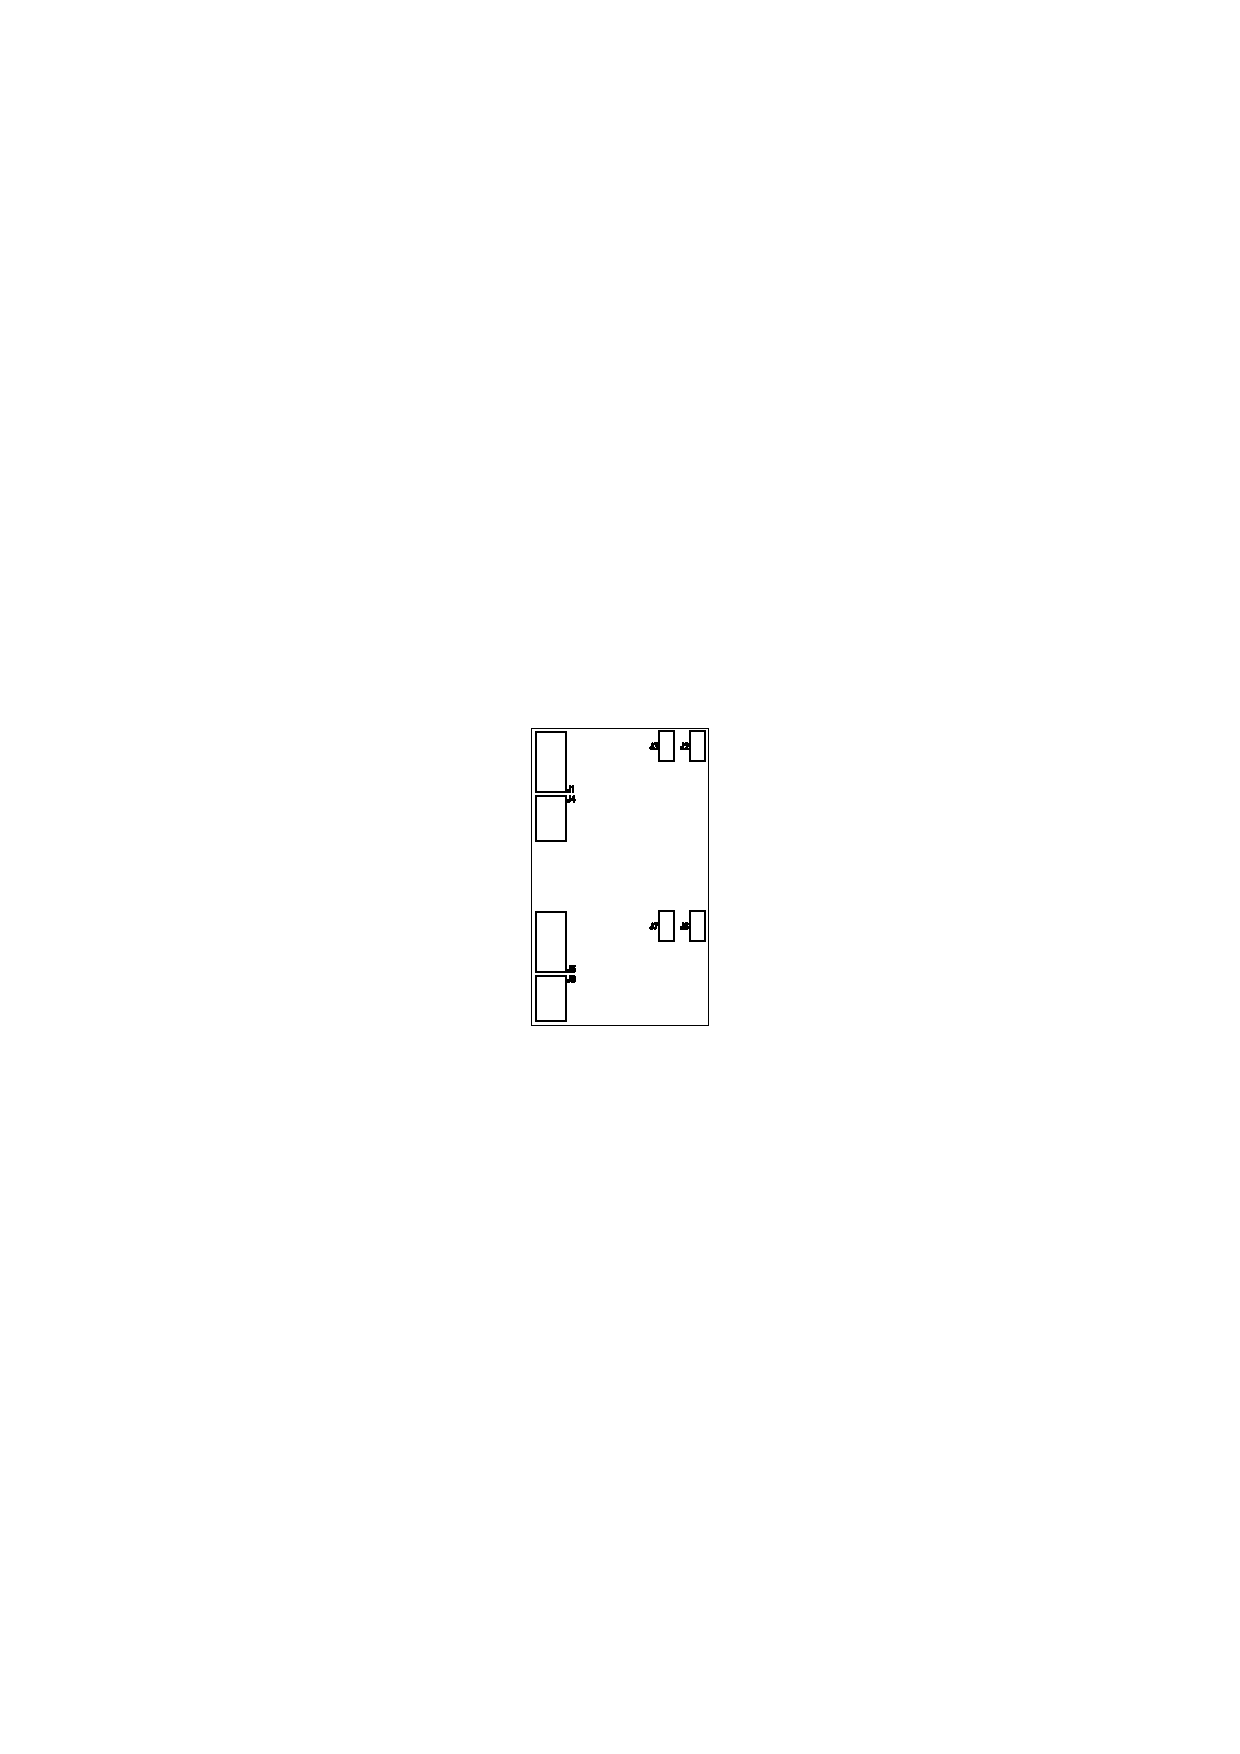
\includegraphics[trim = 6.5cm 11.5cm 6.5cm 11.5cm, clip, width=10cm]{../../CAM_DOC/O2.pdf}
  \caption{Osazovací plán horní a spodní strany plošného spoje}
  \label{fig:osazovaci_plan}
\end{figure}


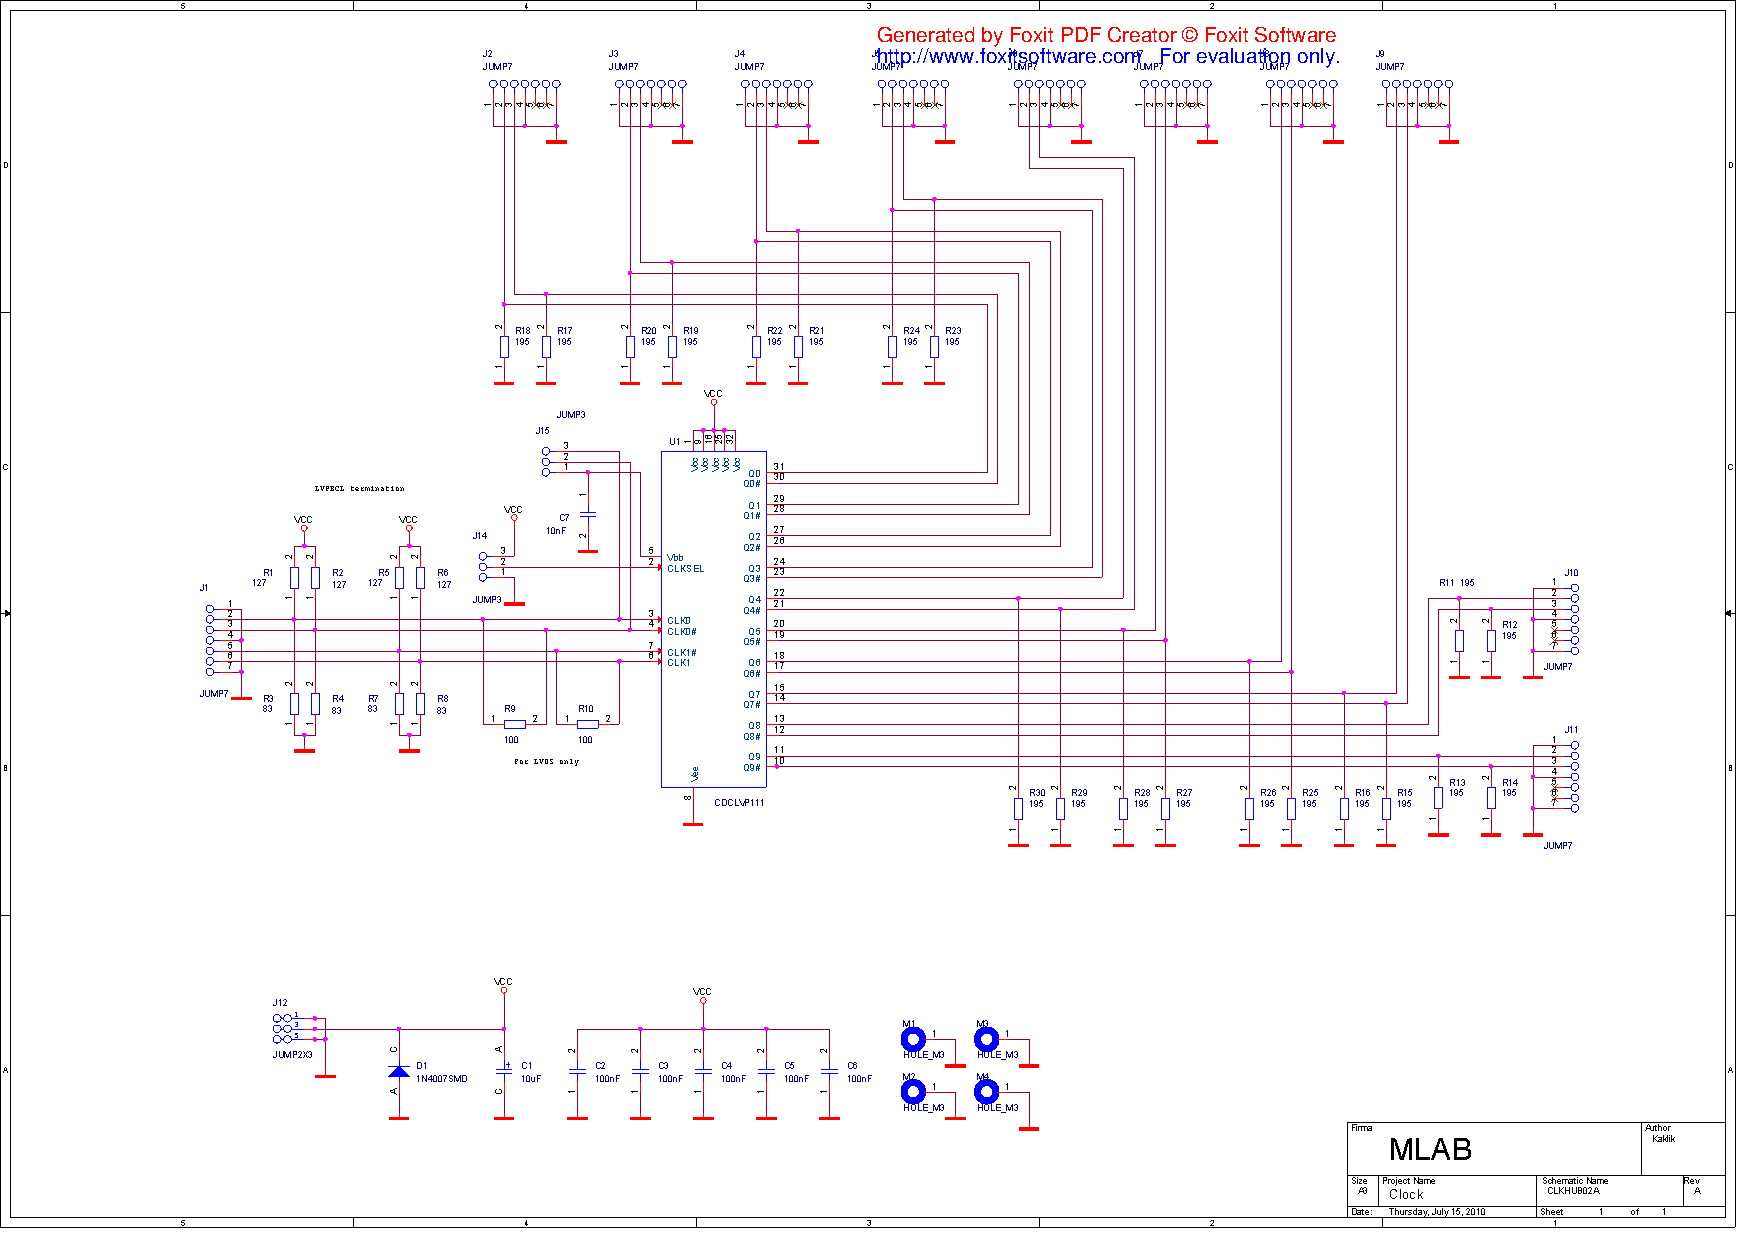
\includepdf[pages={1},landscape=true]{../../SCH/CLKHUB02A.pdf}

Jak je vidět ze zapojení, výstup je předpokládán diferenční v logice PECL. 

\subsection{Odrušení}

Vzhledem k tomu, že modul je ze své podstaty generátorem signálu, je s ním i třeba tak pracovat a dbát na dostatečné odrušení vůči jiným součástem aparatury. Tomuto výrazně pomáhá vhodná volba základní desky, z MLABu nejlépe ALBASE.

\subsection{Mechanická konstrukce}

Modul klasicky předpokládá uchycení na čtyřech šroubech, z důvodu vhodného odstínění je vhodné zabezpečit aby všechny šrouby byly vodivě spojeny s podložkou.  

\section{Výroba a testování}
Modul je z z důvodu zabezpečení kvalitního blokování i na vysokých frekvencích (až 1,5GHz) navržen na dvouvrstvém silně prokoveném plošném spoji. A proto je obtížná jeho amatérská výroba.

\subsubsection{Osazení}

Osazení modulu se liší podle použité diferenční logiky na vstupu modulu. 

\end{document}